\documentclass[aspectratio=169,10pt,t]{beamer}
\usepackage{issa}  % place issa.sty in the same folder
\definecolor{AccentCol}{HTML}{2C3E80}
\renewcommand{\lecnum}{6}
\begin{document}
\titleslide{6}{Reinforcement Learning Part 1:\\Q-Learning \& Deep Q-Networks}{MDPs \textbullet\ Bellman equations \textbullet\ Q-learning \textbullet\ $\varepsilon$-greedy \textbullet\ DQN \textbullet\ replay buffer \textbullet\ reward shaping\\Case study: wargame tactical agent, 20$\times$20 JANUS grid, 100K episodes, 81\% win vs novice human}

\sect{1. Why RL}
\begin{frame}{The Third Paradigm --- Learning by Doing: No Labels, Just Rewards}
\figc{2.6cm}{\begin{tikzpicture}
\tikzset{C/.style={nd,text width=4.6cm,align=left,minimum height=2.3cm,font=\fontsize{6.6}{7.8}\selectfont,inner sep=3pt}}
\node[C,draw=ISSAgrn,fill=ISSAgrn!7]at(-5,0){\textbf{\textcolor{ISSAgrn}{SUPERVISED}}\\Labels $(x,y)$; loss $L(f(x),y)$; static labelled dataset; immediate feedback per sample.\\\textbf{Example:} radar classification.\\\textbf{Weakness:} needs labels; can't exceed the training distribution.};
\node[C,draw=teal,fill=teal!7]at(0,0){\textbf{\textcolor{teal}{UNSUPERVISED}}\\No labels $\{x\}$; reconstruction / likelihood loss; feedback: none, data-driven.\\\textbf{Example:} OPFOR clustering.\\\textbf{Weakness:} no goal direction; can't optimise a specific objective.};
\node[C,draw=AccentCol,fill=AccentCol!8,line width=1.2pt]at(5,0){\textbf{\textcolor{AccentCol}{REINFORCEMENT}}\\Trial and error; loss = negative cumulative reward; data generated by interaction; delayed, sparse feedback.\\\textbf{Example:} wargame tactical agent.\\\textbf{Strength:} learns strategy from experience.};
\end{tikzpicture}}
\begin{columns}[T]
\column{0.50\textwidth}
\figc{2.3cm}{\begin{tikzpicture}
\node[ndN,minimum width=2.6cm,minimum height=0.9cm](a)at(0,0){\textbf{AGENT}\\\sm{policy $\pi(a|s)$}};\node[ndA,minimum width=2.8cm,minimum height=0.9cm](e)at(0,-1.9){\textbf{ENVIRONMENT}\\\sm{wargame simulator}};
\draw[arrA,rounded corners=3pt](a.east)--++(1.0,0)|-node[pos=0.25,right,font=\scriptsize]{action $a_t$}(e.east);\draw[arrA,rounded corners=3pt](e.west)--++(-1.0,0)|-node[pos=0.25,left,font=\scriptsize,align=right]{state $s_{t+1}$\\reward $r_{t+1}$}(a.west);
\end{tikzpicture}}
\column{0.48\textwidth}
\begin{rbox}\scriptsize\textbf{Why RL for defence?} In wargaming and autonomy we cannot label the ``correct'' decision for every battle state (there are $\sim10^{28}$). RL trains by playing millions of simulated games, learning strategic patterns no analyst could pre-specify --- and no human has to label good vs bad moves.\end{rbox}
\end{columns}
\end{frame}

\sect{2. MDPs}
\begin{frame}{Markov Decision Process --- Five Elements Define the Agent's World}
\begin{columns}[T]
\column{0.52\textwidth}
\begin{cbox}{$(S,A,P,R,\gamma)$}\scriptsize
\textbf{$S$ --- state space:} unit positions, resources, OPFOR positions, terrain, weather, ammo, morale: $20\times20$ grid $\times$ resources $\times$ OPFOR $\approx10^{28}$ states.\\[2pt]
\textbf{$A$ --- action space:} \{move N, S, E, W, attack, defend, resupply\} = 7 per unit; 8 units $\Rightarrow7^{8}=5.8$M joint options per turn.\\[2pt]
\textbf{$P(s'|s,a)$ --- transitions:} set by the combat-resolution model (terrain, weather, unit quality).\\[2pt]
\textbf{$R(s,a,s')$ --- reward:} $+10$ capture objective, $+5$ destroy enemy unit, $-8$ lose friendly unit.\\[2pt]
\textbf{$\gamma$ --- discount:} weight on future reward.\end{cbox}
\begin{fbx}{Return to maximise}\[G_t=\sum_{k=0}^{\infty}\gamma^{k}r_{t+k+1}\]\end{fbx}
\column{0.46\textwidth}
\figc{3.2cm}{\begin{tikzpicture}[x=0.42cm,y=0.42cm]
\foreach \i in {0,...,9}{\foreach \jj in {0,...,7}{\draw[ISSAgrey!60](\i,\jj)rectangle++(1,1);}}
\foreach \i/\jj in {3/2,3/3,3/4,6/5,7/5}{\fill[ISSAgrn!40](\i,\jj)rectangle++(1,1);}
\fill[ISSAamb!50](8,6)rectangle++(1,1);\node[font=\tiny\bfseries]at(8.5,6.5){OBJ};
\node[circle,fill=ISSAblue,inner sep=2pt]at(1.5,1.5){};\node[circle,fill=ISSAblue,inner sep=2pt]at(2.5,0.5){};
\node[circle,fill=ISSAred,inner sep=2pt]at(6.5,3.5){};\node[circle,fill=ISSAred,inner sep=2pt]at(7.5,2.5){};
\draw[arrA](1.5,1.5)--(1.5,2.5);\draw[arrA](1.5,1.5)--(2.4,1.5);
\node[lab,anchor=west]at(0,-0.6){\textcolor{ISSAblue}{$\bullet$} Blue \ \textcolor{ISSAred}{$\bullet$} OPFOR \ green = cover};
\end{tikzpicture}}
\begin{ibox}\scriptsize\textbf{Discount intuition:} with $\gamma=0.95$ a reward 14 turns away is worth $0.95^{14}\approx0.49$ of an immediate one --- the agent cares about the future, but not infinitely.\end{ibox}
\end{columns}
\end{frame}

\begin{frame}{The Markov Property --- and Why Real Warfare Is a POMDP}
\begin{columns}[T]
\column{0.50\textwidth}
\begin{fbx}{Markov property}\[P(s_{t+1}\mid s_t,a_t,s_{t-1},a_{t-1},\ldots)=P(s_{t+1}\mid s_t,a_t)\]\end{fbx}
\begin{tl}\item The future depends only on the \textbf{present} state, not the whole history\item If it holds, the agent need not remember all past decisions --- the current state suffices for optimal action\item So the state must encode EVERYTHING relevant: ammo, morale, previous attrition, known OPFOR dispositions, intelligence quality\end{tl}
\begin{wbox}\scriptsize If relevant information is missing from the state, the problem becomes a \textbf{POMDP} (partially observable MDP) --- harder: the agent must maintain a \emph{belief} over the true state. Real warfare is almost certainly a POMDP.\end{wbox}
\column{0.48\textwidth}
\figc{3.0cm}{\begin{tikzpicture}
\node[ndN,minimum width=2.2cm](s)at(0,1.4){true state $s_t$\\\sm{all OPFOR positions}};\node[nd,minimum width=2.2cm](o)at(0,0){observation $o_t$\\\sm{sensor picture, partial}};\node[ndA,minimum width=2.4cm](b)at(3.4,0){belief $b_t(s)$\\\sm{probability over states}};\node[ndG,minimum width=1.6cm](a)at(3.4,1.4){action $a_t$};
\draw[arr](s)--node[left,lab]{fog of war}(o);\draw[arr](o)--(b);\draw[arr](b)--(a);\draw[arr,dashed](a)--(s);
\end{tikzpicture}}
\begin{ibox}\scriptsize\textbf{Simplification:} most wargame RL systems assume full observability (known OPFOR positions) --- a major assumption that limits real-world transfer. Lecture 8 returns to partial observability for multi-agent teams.\end{ibox}
\end{columns}
\end{frame}

\sect{3. Bellman Equations}
\begin{frame}{Bellman Equations --- Recursive Characterisation of the Optimal Policy}
\begin{columns}[T]
\column{0.52\textwidth}
\begin{fbx}{Bellman optimality}\[V^{*}(s)=\max_a\sum_{s'}P(s'|s,a)\big[R(s,a,s')+\gamma V^{*}(s')\big]\]\[Q^{*}(s,a)=\sum_{s'}P(s'|s,a)\big[R(s,a,s')+\gamma\max_{a'}Q^{*}(s',a')\big]\]\[V^{*}(s)=\max_aQ^{*}(s,a),\qquad\pi^{*}(s)=\arg\max_aQ^{*}(s,a)\]\end{fbx}
\begin{tl}\item ``The value of $s$ = the best action's expected immediate reward PLUS discounted future value''\item Policy evaluation: $V^\pi(s)=\sum_a\pi(a|s)\sum_{s'}P(s'|s,a)[R+\gamma V^\pi(s')]$; $V^{*}$ = max over policies\item If we know $Q^{*}$, the optimal policy is trivial: take $\arg\max_aQ^{*}(s,a)$ --- the goal of Q-learning\end{tl}
\column{0.46\textwidth}
\subhead{Backup diagram}
\figc{3.3cm}{\begin{tikzpicture}
\node[circle,draw=AccentCol,fill=AccentCol!20,minimum size=0.7cm,font=\scriptsize](s)at(0,0){$s$};
\foreach \x/\nm/\l in {-1.8/aA/a_1,0/aB/a_2,1.8/aC/a_3}{\node[circle,fill=black,inner sep=2pt](\nm)at(\x,-1.2){};\draw(s)--(\nm);\node[font=\tiny,anchor=east]at(\x-0.05,-1.0){$\l$};}
\foreach \x/\p in {-2.4/aA,-1.2/aA,-0.6/aB,0.6/aB,1.2/aC,2.4/aC}{\node[circle,draw=AccentCol,minimum size=0.5cm,font=\tiny](t)at(\x,-2.5){$s'$};\draw(\p)--(t);}
\draw[ISSAred,thick](-2.2,-1.45)--(2.2,-1.45);\node[font=\tiny,ISSAred,anchor=west]at(2.2,-1.45){max over $a$};
\node[font=\tiny,anchor=west]at(2.7,-2.5){average over $s'$ (weighted by $P$)};
\end{tikzpicture}}
\sm{Value flows back up the tree: average over what the environment does, maximise over what the agent does.}
\end{columns}
\end{frame}

\begin{frame}{Wargame Worked Example --- Reading Q-Values}
\begin{columns}[T]
\column{0.52\textwidth}
\begin{cbox}[ISSAnavy]{State $s$}\scriptsize Blue unit adjacent to enemy; ammo HIGH; morale HIGH; terrain COVER; objective nearby. Q-values from the trained model:\end{cbox}
\figc{3.3cm}{\begin{tikzpicture}\begin{axis}[xbar,width=7.0cm,height=4.0cm,symbolic y coords={Move W,Move S,Resupply,Move E,Defend,Move N,Attack},ytick=data,xmin=0,xmax=21,bar width=7pt,nodes near coords,nodes near coords style={font=\fontsize{5.5}{6}\selectfont},xlabel={$Q(s,a)$},xmajorgrids]
\addplot[fill=AccentCol!45]coordinates{(3.2,Move W)(4.8,Move S)(6.1,Resupply)(8.1,Move E)(9.2,Defend)(12.4,Move N)};\addplot[fill=ISSAgrn!80,bar shift=0pt]coordinates{(18.7,Attack)};
\end{axis}\end{tikzpicture}}
\column{0.46\textwidth}
\begin{rbox}\scriptsize\textbf{Optimal action:} $\pi^{*}(s)=\arg\max_a Q=\textbf{ATTACK}$ (18.7).\end{rbox}
\begin{cbox}{What the numbers mean}\scriptsize $Q^{*}(s,\text{Attack})=18.7$: expected cumulative \emph{discounted reward} from $s$ if I attack now and then play optimally from every later state. $Q^{*}(s,\text{Defend})=9.2$: defending yields less total reward in this specific state (high ammo, in cover).\end{cbox}
\begin{wbox}\scriptsize\textbf{Interpretation pitfall:} Q-values are in \emph{reward units}, not probabilities. ``18.7'' does not mean ``18.7\% chance of winning''.\end{wbox}
\end{columns}
\end{frame}

\sect{4. Q-Learning}
\begin{frame}{Q-Learning (Watkins, 1989) --- Model-Free, Off-Policy TD Control}
\begin{columns}[T]
\column{0.50\textwidth}
\begin{fbx}{TD update rule}\[Q(s,a)\leftarrow Q(s,a)+\alpha\big[\underbrace{r+\gamma\max_{a'}Q(s',a')}_{\text{TD target}}-Q(s,a)\big]\]\[\delta=r+\gamma\max_{a'}Q(s',a')-Q(s,a)\quad\text{(TD error)}\]\end{fbx}
\begin{tl}\item \textbf{Model-free:} no need to know $P(s'|s,a)$ or $R$ in advance; learns $Q^{*}$ from interaction\item $\alpha\in(0,1]$ learning rate; ``shift the estimate toward the target by a fraction $\alpha$ of the error''\item \textbf{Off-policy:} uses $\max_{a'}$ (the greedy next action) regardless of the action actually taken next\end{tl}
\column{0.48\textwidth}
\subhead{Numerical walk-through ($\alpha=0.1$, $\gamma=0.9$)}
\figc{1.9cm}{\begin{tikzpicture}
\node[ndN,minimum width=1.8cm](s1)at(0,0){$s_1$\\\sm{2 hexes from objective}};\node[ndG,minimum width=1.8cm](s2)at(4.2,0){$s_2$\\\sm{adjacent to objective}};
\draw[bigarr](s1)--node[above,font=\tiny]{MOVE N, $r=0$}node[below,font=\tiny]{$Q(s_1,\text{N})=5.0$}(s2);
\node[font=\tiny,anchor=west]at(5.2,0.25){$Q(s_2,\text{ATTACK})=14.2$};\node[font=\tiny,anchor=west]at(5.2,-0.2){$Q(s_2,\text{MOVE N})=8.1$};
\end{tikzpicture}}
\begin{cbox}[ISSAgrn]{One update}\scriptsize TD target $=0+0.9\times14.2=12.78$; TD error $\delta=12.78-5.0=7.78$ (positive: MOVE N was undervalued because it leads to a high-value state). New $Q(s_1,\text{N})=5.0+0.1\times7.78=\mathbf{5.778}$. After 1,000 episodes $\approx11.8$, converging toward 12.78.\end{cbox}
\end{columns}
\end{frame}

\begin{frame}{$\varepsilon$-Greedy Exploration --- the Exploration--Exploitation Dilemma}
\begin{columns}[T]
\column{0.50\textwidth}
\begin{fbx}{$\varepsilon$-greedy policy and annealing}\[P(a=a^{*})=(1-\varepsilon)+\tfrac{\varepsilon}{|A|},\qquad P(a\ne a^{*})=\tfrac{\varepsilon}{|A|}\]\[\varepsilon_t=\varepsilon_{\min}+(\varepsilon_{\max}-\varepsilon_{\min})\,e^{-t/\tau}\]\end{fbx}
\begin{tl}\item With probability $\varepsilon$: EXPLORE (random action); otherwise EXPLOIT ($\arg\max Q$)\item Start $\varepsilon=1.0$ (know nothing); end $\varepsilon=0.05$ (mostly exploit, keep 5\% exploring); typical wargame $\tau=5{,}000$ episodes\end{tl}
\column{0.48\textwidth}
\figc{3.0cm}{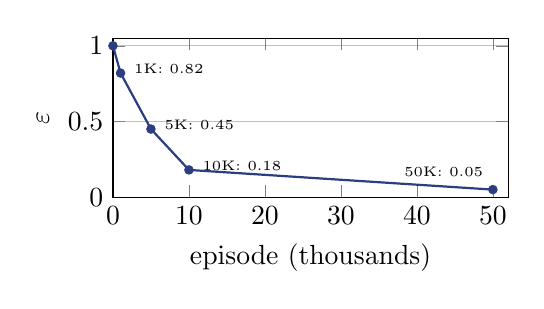
\begin{tikzpicture}\begin{axis}[width=6.6cm,height=3.6cm,xlabel={episode (thousands)},ylabel={$\varepsilon$},xmin=0,xmax=52,ymin=0,ymax=1.05,ymajorgrids]
\addplot[AccentCol,thick,mark=*,mark size=1.3pt]coordinates{(0,1.00)(1,0.82)(5,0.45)(10,0.18)(50,0.05)};
\node[font=\tiny,anchor=west]at(axis cs:1.5,0.85){1K: 0.82};\node[font=\tiny,anchor=west]at(axis cs:5.5,0.48){5K: 0.45};\node[font=\tiny,anchor=west]at(axis cs:10.5,0.21){10K: 0.18};\node[font=\tiny,anchor=south east]at(axis cs:50,0.07){50K: 0.05};
\end{axis}\end{tikzpicture}}
\sm{Case-study schedule (as reported).}
\begin{ibox}\scriptsize A commander faces the same dilemma: keep using the tactic that has worked, or probe an untried approach that might work better. Never exploring locks in a sub-optimal habit.\end{ibox}
\end{columns}
\end{frame}

\begin{frame}{Q-Learning Convergence --- the Theory and the Tabular Wall}
\begin{columns}[T]
\column{0.50\textwidth}
\begin{cbox}{Theorem (Watkins \& Dayan, 1992)}\scriptsize Q-learning converges to $Q^{*}$ with probability 1 if: \textcircled{\tiny1} every $(s,a)$ is visited infinitely often ($\varepsilon>0$); \textcircled{\tiny2} learning rates satisfy Robbins--Monro: $\sum_t\alpha_t=\infty$, $\sum_t\alpha_t^2<\infty$ (e.g.\ $\alpha_t=1/t$); \textcircled{\tiny3} stationary rewards; \textcircled{\tiny4} finite state--action space.\end{cbox}
\begin{ibox}\scriptsize\textbf{In practice:} a small constant $\alpha$ (e.g.\ 0.001) --- theoretically non-convergent, but it works well and adapts to non-stationary environments.\end{ibox}
\begin{wbox}\scriptsize\textbf{Tabular limitation:} Q-table size $=|S|\times|A|$. For the wargame $10^{28}\times7$ --- impossible to store or enumerate. Solution: \textbf{function approximation} --- replace the table with a neural network $Q(s,a;\theta)$: the DQN.\end{wbox}
\column{0.48\textwidth}
\figc{3.1cm}{\begin{tikzpicture}\begin{axis}[width=6.6cm,height=3.7cm,xlabel={training episodes (thousands)},ylabel={win rate vs random (\%)},xmin=0,xmax=105,ymin=0,ymax=100,ymajorgrids]
\addplot[AccentCol,thick,mark=*]coordinates{(0,14)(10,38)(50,76)(100,91)};
\node[font=\tiny,anchor=north west]at(axis cs:11,38){38\%};\node[font=\tiny,anchor=north west]at(axis cs:51,76){76\%};\node[font=\tiny,anchor=south east]at(axis cs:100,92){91\%};
\fill[ISSAred!12](axis cs:0,0)rectangle(axis cs:20,100);\node[font=\tiny,anchor=north]at(axis cs:10,98){exploration};
\end{axis}\end{tikzpicture}}
\sm{DQN on the 20$\times$20 grid (as reported: 10K 38\%, 50K 76\%, 100K 91\%); the episode-0 point is illustrative. Phases: 0--20K random-like, 20--60K rapid improvement, then refinement.}
\end{columns}
\end{frame}

\sect{5. Deep Q-Networks}
\begin{frame}{Deep Q-Network --- Replace the Q-Table with a Neural Network}
\begin{columns}[T]
\column{0.52\textwidth}
\figc{2.8cm}{\begin{tikzpicture}
\foreach \x/\h/\lbl in {0/2.6/410,1.6/2.2/512,3.2/2.2/512,4.8/1.0/7}{\fill[AccentCol!20,draw=AccentCol](\x-0.3,-\h/2)rectangle(\x+0.3,\h/2);\node[font=\tiny]at(\x,-\h/2-0.2){\lbl};}
\foreach \a/\b/\ha/\hb in {0/1.6/2.6/2.2,1.6/3.2/2.2/2.2,3.2/4.8/2.2/1.0}{\draw[ISSAgrey](\a+0.3,\ha/2)--(\b-0.3,\hb/2);\draw[ISSAgrey](\a+0.3,-\ha/2)--(\b-0.3,-\hb/2);}
\node[lab]at(0,1.55){state $s$};\node[lab]at(1.6,1.35){FC1 ReLU};\node[lab]at(3.2,1.35){FC2 ReLU};\node[lab,anchor=west]at(5.2,0){$Q(s,a_1;\theta)\ldots Q(s,a_7;\theta)$};
\end{tikzpicture}}
\begin{tl}\item Input: 400-dim grid encoding + unit attributes (ammo, HP, morale) $=$ 410 features\item One forward pass $\to$ all 7 Q-values; parameters $410\cdot512+512\cdot512+512\cdot7=479{,}744$\item Adam, lr 0.0001 (Mnih et al., 2015 style)\end{tl}
\column{0.46\textwidth}
\begin{fbx}{DQN loss}\[L(\theta)=\mathbb{E}\big[(y-Q(s,a;\theta))^{2}\big]\]\[y=r+\gamma\max_{a'}Q(s',a';\theta^{-})\]\end{fbx}
\begin{tl}\item $\theta$: online network, trained by SGD\item $\theta^{-}$: \textbf{target network}, a frozen copy used only to compute $y$\end{tl}
\begin{ibox}\scriptsize Generalisation is the whole point: states never visited still get sensible Q-values because similar states share network weights --- impossible with a table.\end{ibox}
\end{columns}
\end{frame}

\begin{frame}{DQN's Two Key Innovations --- Experience Replay and the Target Network}
\begin{columns}[T]
\column{0.50\textwidth}
\figc{2.3cm}{\begin{tikzpicture}
\node[ndN](env)at(0,0){agent + env};\node[nd,minimum width=2.4cm,minimum height=1.1cm](buf)at(3.0,0){\textbf{Replay buffer $D$}\\\sm{100,000 transitions}\\\sm{$(s,a,r,s',\text{done})$}};\node[ndA](mb)at(6.0,0){random\\mini-batch 32};
\draw[arr](env)--node[above,font=\tiny]{store}(buf);\draw[arr](buf)--node[above,font=\tiny]{sample}(mb);\draw[arr,dashed](mb.south)--++(0,-0.5)-|node[pos=0.25,below,font=\tiny]{SGD update of $\theta$}(env.south);
\end{tikzpicture}}
\begin{cbox}[ISSAgrn]{Innovation 1: experience replay}\scriptsize \textcircled{\tiny1} breaks temporal correlation between consecutive samples (correlated updates cause divergence); \textcircled{\tiny2} each experience is reused $\sim$1,000 times (sample efficiency); \textcircled{\tiny3} stabilises training dramatically.\end{cbox}
\column{0.48\textwidth}
\figc{2.3cm}{\begin{tikzpicture}
\node[ndN,minimum width=2.2cm](on)at(0,0){online net $\theta$\\\sm{updated every step}};\node[ndA,minimum width=2.2cm](tg)at(3.6,0){target net $\theta^{-}$\\\sm{frozen}};\draw[arr,dashed](on)--node[above,font=\tiny]{copy every $C=1{,}000$ steps}(tg);\node[nd](y)at(3.6,-1.3){$y=r+\gamma\max Q(s',a';\theta^{-})$};\draw[arr](tg)--(y);\draw[arr](y)-|(on);
\end{tikzpicture}}
\begin{cbox}[ISSAblue]{Innovation 2: the target network}\scriptsize Without it, the target $y$ moves every time $\theta$ changes --- chasing a moving target $\Rightarrow$ instability. Frozen $\theta^{-}$ keeps the target stable for $C$ steps.\end{cbox}
\begin{wbox}\scriptsize Without both innovations, DQN often diverges (vanilla DQN: 74\% vs random and unstable).\end{wbox}
\end{columns}
\end{frame}

\begin{frame}{Double DQN and Dueling DQN --- Better Value Estimates}
\begin{columns}[T]
\column{0.50\textwidth}
\subhead{Double DQN (van Hasselt 2016): fix overestimation}
\begin{fbx}{Decouple selection from evaluation}\[a^{*}=\arg\max_{a'}Q(s',a';\theta),\qquad y=r+\gamma Q(s',a^{*};\theta^{-})\]\end{fbx}
\sm{Standard DQN's $\max$ picks the noisiest estimate, so Q-values are systematically too high and the agent becomes over-confident on rare states. One network picks; the other scores.}
\figc{2.0cm}{\bars{20}{1.4}{2.2}{Standard DQN overestimation/18.4/ISSAred,Double DQN overestimation/4.2/ISSAgrn}}
\sm{Average overestimation after 50K episodes (reward units).}
\column{0.48\textwidth}
\subhead{Dueling DQN (Wang 2016): value + advantage}
\figc{2.4cm}{\begin{tikzpicture}
\node[nds,minimum width=1.3cm](in)at(0,0){state};\node[ndN,minimum width=1.5cm](sh)at(1.9,0){shared\\\sm{512$\to$256}};\node[ndA](v)at(4.0,0.6){$V(s)$\\\sm{1 output}};\node[ndA](ad)at(4.0,-0.6){$A(s,a)$\\\sm{7 outputs}};\node[ndG](q)at(6.3,0){$Q=V+A-\bar A$};
\draw[arr](in)--(sh);\draw[arr](sh)--(v);\draw[arr](sh)--(ad);\draw[arr](v)--(q);\draw[arr](ad)--(q);
\end{tikzpicture}}
\begin{fbx}{Decomposition}\[Q(s,a)=V(s)+A(s,a)-\tfrac{1}{|A|}\sum_{a'}A(s,a')\]\end{fbx}
\sm{$V$: how good is the state regardless of action? $A$: how much better is $a$ than average? Subtracting the mean makes $V$ and $A$ identifiable. Helps in states where all moves are similar (no enemy near).}
\end{columns}
\end{frame}

\sect{6. Rewards \& Curriculum}
\begin{frame}{Reward Shaping --- When +100 Win / $-$100 Lose Is Too Sparse to Learn From}
\begin{columns}[T]
\column{0.50\textwidth}
\begin{wbox}\scriptsize\textbf{Naive reward:} $+100$ win, $-100$ lose, 0 otherwise. Games last $\sim$40 turns, so 40 actions get no feedback; early on the agent almost always loses --- all $-100$s, no gradient. Result: a random policy for the first 20,000+ episodes.\end{wbox}
\begin{fbx}{Potential-based shaping (Ng, Harada \& Russell 1999)}\[R_{\text{shaped}}=R(s,a,s')+F(s,s'),\qquad F=\gamma\Phi(s')-\Phi(s)\]\end{fbx}
\sm{$\Phi(s)$ estimates ``how good is $s$''. Potential-based shaping adds guidance WITHOUT changing the optimal policy.}
\column{0.48\textwidth}
\subhead{Wargame shaping rewards}
\figc{2.8cm}{\begin{tikzpicture}[x=0.27cm,y=0.42cm]
\draw[ISSAdark!60](0,0.6)--(0,-4.6);
\foreach \i/\lbl/\v in {0/Capture objective/10,1/Destroy enemy unit/5,2/Move toward objective/2}{\fill[ISSAgrn!70](0,-\i-0.35)rectangle(\v,-\i+0.35);\node[font=\fontsize{5.8}{6}\selectfont,anchor=west]at(\v+0.3,-\i){\lbl\ (+\v)};}
\foreach \i/\lbl/\v in {3/Lose friendly unit/8}{\fill[ISSAred!70](-\v,-\i-0.35)rectangle(0,-\i+0.35);\node[font=\fontsize{5.8}{6}\selectfont,anchor=west]at(0.3,-\i){\lbl\ ($-$\v)};}
\end{tikzpicture}}
\begin{ibox}\scriptsize\textbf{Danger:} badly designed shaping teaches the agent to farm the bonus (e.g.\ circling near the objective to collect ``move toward'' rewards) instead of winning. Keep shaping potential-based and audit agent behaviour.\end{ibox}
\end{columns}
\end{frame}

\begin{frame}{Curriculum Learning --- Start Simple, Add Complexity}
\begin{columns}[T]
\column{0.54\textwidth}
\figc{3.5cm}{\begin{tikzpicture}\begin{axis}[width=7.4cm,height=4.1cm,xlabel={training episode (thousands)},ylabel={win rate (\%)},xmin=0,xmax=100,ymin=40,ymax=100,ymajorgrids,legend pos=south east]
\addplot[AccentCol,thick,mark=*]coordinates{(5,72)};\addplot[AccentCol,thick,mark=*]coordinates{(5,68)(20,84)};\addplot[AccentCol,thick,mark=*]coordinates{(20,54)(60,79)};\addplot[AccentCol,thick,mark=*]coordinates{(60,79)(100,91)};
\addplot[ISSAred,thick,dashed,mark=square*]coordinates{(0,45)(100,51)};
\node[font=\tiny,anchor=south]at(axis cs:5,73){P1 5$\times$5};\node[font=\tiny,anchor=south]at(axis cs:13,85){P2 10$\times$10};\node[font=\tiny,anchor=north]at(axis cs:40,62){P3 20$\times$20};\node[font=\tiny,anchor=south]at(axis cs:84,92){P4 full + adaptive};\node[font=\tiny,ISSAred,anchor=north]at(axis cs:80,50){no curriculum: 51\%};
\end{axis}\end{tikzpicture}}
\sm{Each phase transfers weights to the next; the drops at phase starts are the harder scenario, not forgetting. The no-curriculum start value is illustrative.}
\column{0.44\textwidth}
\begin{cbox}{The wargame curriculum}\scriptsize \textbf{P1 (0--5K):} 5$\times$5, 1 v 1, fixed positions; a Q-table works: 72\%. \textbf{P2 (5--20K):} 10$\times$10, 3 v 3, two terrain types; transfer to DQN: 68\%$\to$84\%. \textbf{P3 (20--60K):} 20$\times$20, 8 v 8, 5 terrains + weather: 54\%$\to$79\%. \textbf{P4 (60--100K):} full + adaptive OPFOR: 79\%$\to$91\% vs random; 63\%$\to$81\% vs novice human.\end{cbox}
\begin{rbox}\scriptsize\textbf{Key result:} trained directly on the full scenario, DQN reached only \textbf{51\%} after 100K episodes vs \textbf{91\%} with the curriculum --- a 40-point gain. Like cadets: drills before battles.\end{rbox}
\end{columns}
\end{frame}

\sect{7. Case Study Results}
\begin{frame}{Wargame Case Study --- DQN Agent on the 20$\times$20 JANUS Hex Grid}
\begin{columns}[T]
\column{0.58\textwidth}
\figc{3.6cm}{\scriptsize\renewcommand{\arraystretch}{1.13}\begin{tabular}{llccl}\toprule\textbf{Algorithm}&\textbf{Opponent}&\textbf{Win}&\textbf{Turns}&\textbf{Notes}\\\midrule Tabular Q (10$\times$10)&random&91\%&22.4&table infeasible at 20$\times$20\\DQN (vanilla)&random&74\%&31.8&no replay/target: unstable\\DQN + replay&random&83\%&28.2&replay alone stabilises\\DQN + replay + target&random&88\%&26.7&stable convergence\\Double DQN&random&91\%&25.1&overestimation corrected\\\rowcolor{ISSAgrn!20}Dueling + Double&random&\textbf{93\%}&23.8&best vs random\\Dueling + Double&novice human&81\%&29.4&human adapts\\Dueling + Double&minimax AI&54\%&38.2&classical AI competitive\\\bottomrule\end{tabular}}
\sm{All DQN variants: 100K training episodes; tabular Q: 50K.}
\column{0.40\textwidth}
\figc{3.0cm}{\bars{100}{2.0}{1.2}{Vanilla/74/ISSAred,+Replay/83/ISSAamb,+Target/88/ISSAblue,Double/91/AccentCol,Dueling + Double/93/ISSAgrn}}
\sm{Win rate vs random OPFOR (\%).}
\begin{ibox}\scriptsize Each stabilisation trick adds measurable performance --- but the opponent matters more than the algorithm: 93\% $\to$ 81\% $\to$ 54\%.\end{ibox}
\end{columns}
\end{frame}

\begin{frame}{Sim-to-Real Gap and the Advisory Role of Wargame AI}
\begin{columns}[T]
\column{0.50\textwidth}
\figc{2.4cm}{\bars{100}{1.7}{2.0}{vs random OPFOR/93/ISSAgrn,vs novice human/81/ISSAamb,vs minimax AI/54/ISSAred}}
\begin{wbox}\scriptsize\textbf{Sim-to-real warning:} 91\% vs random OPFOR in simulation $\neq$ 91\% in a field exercise. Human OPFOR adapts, introduces friction, and exploits the AI's pattern repetition. Minimax at 54\% shows classical adversarial search remains highly competitive --- DQN is not a solved problem for wargame AI.\end{wbox}
\column{0.48\textwidth}
\subhead{Recommended role: ADVISOR, not commander}
\figc{2.6cm}{\begin{tikzpicture}
\node[draw=AccentCol,fill=white,rounded corners=2pt,minimum width=5.6cm,minimum height=2.6cm](p)at(0,0){};
\node[font=\scriptsize\bfseries,AccentCol,anchor=north west]at(-2.7,1.2){AI ADVISOR --- Unit B3};
\foreach \i/\a/\q/\w in {0/ATTACK/18.7/3.1,1/MOVE N/12.4/2.1,2/DEFEND/9.2/1.5}{\node[font=\scriptsize,anchor=west]at(-2.6,0.55-\i*0.5){\i.\ \a};\fill[AccentCol!60](-0.6,0.42-\i*0.5)rectangle(-0.6+\w*0.6,0.68-\i*0.5);\node[font=\tiny,anchor=west]at(-0.55+\w*0.6,0.55-\i*0.5){$Q$ = \q};}
\node[ndG,font=\tiny,minimum height=0.32cm,inner sep=1.5pt]at(1.6,-1.0){commander decides};
\end{tikzpicture}}
\sm{Mock-up: top-3 actions with Q-values; the human selects.}
\begin{rbox}\scriptsize\textbf{Operational insight:} propose the top-3 actions with their Q-values and let the commander choose. Human + AI outperforms either alone.\end{rbox}
\end{columns}
\end{frame}

\sect{8. Across Disciplines}
\begin{frame}{Reinforcement Learning Across the Disciplines}
\subhead{Reward-driven learning was discovered in animals, formalised for the military, and proven in games}
\figc{5.0cm}{\begin{tikzpicture}
\tikzset{G/.style={nd,text width=4.75cm,align=left,minimum height=2.3cm,font=\fontsize{6.9}{8.2}\selectfont,inner sep=3pt}}
\node[G,draw=violet,fill=violet!7]at(-5,1.25){\textbf{\textcolor{violet}{PSYCHOLOGY}}\\Thorndike's law of effect (1898) and Skinner's operant conditioning: actions followed by reward are repeated --- the behavioural root of RL.\\\textbf{Defence:} training design --- immediate, consistent feedback speeds skill acquisition, as reward shaping does for agents.};
\node[G,draw=ISSAgrn,fill=ISSAgrn!7]at(0,1.25){\textbf{\textcolor{ISSAgrn}{BIOLOGY / NEUROSCIENCE}}\\Dopamine neurons fire in proportion to the \emph{reward-prediction error} --- almost exactly the TD error $\delta$ (Schultz, Dayan \& Montague, \textit{Science}, 1997).\\\textbf{Lesson:} Q-learning's update mirrors how brains learn.};
\node[G,draw=ISSAred,fill=ISSAred!6]at(5,1.25){\textbf{\textcolor{ISSAred}{ENGINEERING / OR}}\\Richard Bellman developed dynamic programming at the RAND Corporation in the 1950s --- the Bellman equation came from defence-funded operations research.\\\textbf{Defence:} optimal control, logistics scheduling, missile guidance.};
\node[G,draw=ISSAblue,fill=ISSAblue!7]at(-5,-1.25){\textbf{\textcolor{ISSAblue}{AERONAUTICS}}\\RL controllers learned to fly a model helicopter through aerobatic manoeuvres, including sustained inverted flight (Ng et al., Stanford, 2004).\\\textbf{Defence:} autonomous flight control under turbulence --- the theme of Lecture 7.};
\node[G,draw=ISSAamb,fill=ISSAyell!45]at(0,-1.25){\textbf{\textcolor{ISSAamb!80!black}{STATISTICS}}\\Thompson (1933) proposed allocating treatments in clinical trials by posterior probability --- the multi-armed bandit, origin of the exploration--exploitation trade-off.\\\textbf{Defence:} sensor tasking: keep watching known emitters or search for new ones?};
\node[G,draw=AccentCol,fill=AccentCol!8]at(5,-1.25){\textbf{\textcolor{AccentCol}{GAMES \& WARGAMING}}\\TD-Gammon (Tesauro, 1990s) reached expert backgammon by self-play; in DARPA's AlphaDogfight Trials (2020) an RL agent beat an experienced F-16 pilot 5--0 in simulation.\\\textbf{Caution:} simulation victories are not combat victories.};
\end{tikzpicture}}
\begin{ibox}\scriptsize\textbf{Common thread:} learn from consequences, balance exploring against exploiting, and beware of rewarding the wrong thing --- in animals, organisations and agents alike.\end{ibox}
\end{frame}

\sect{9. Summary}
\begin{frame}{Lecture 6 Summary --- From MDP Formalism to Wargame Tactical Agents}
\figc{4.9cm}{\begin{tikzpicture}
\tikzset{K/.style={nd,text width=3.6cm,align=left,minimum height=2.1cm,font=\fontsize{6.4}{7.6}\selectfont,inner sep=3pt}}
\node[K,draw=ISSAblue,fill=ISSAblue!8]at(-4,1.2){\textbf{MDP FORMALISM}\\$(S,A,P,R,\gamma)$; Markov property: the future depends on the present; wargame $\sim10^{28}$ states $\Rightarrow$ DQN.\\\textbf{First:} define the problem};
\node[K,draw=ISSAgrn,fill=ISSAgrn!8]at(0,1.2){\textbf{BELLMAN EQUATIONS}\\$Q^{*}(s,a)=\sum P[R+\gamma\max Q^{*}]$; $\pi^{*}=\arg\max Q^{*}$; Q-values are reward units, not probabilities.\\\textbf{Core:} recursive optimality};
\node[K,draw=violet,fill=violet!8]at(4,1.2){\textbf{Q-LEARNING}\\$Q\leftarrow Q+\alpha[r+\gamma\max Q'-Q]$; model-free, off-policy, convergent (tabular); sparse reward slows it.\\\textbf{Core:} the update rule};
\node[K,draw=AccentCol,fill=AccentCol!10]at(-4,-1.2){\textbf{DQN INNOVATIONS}\\Experience replay breaks correlations; target network stabilises targets; without both, training often diverges.\\\textbf{Essential:} for stability};
\node[K,draw=ISSAamb,fill=ISSAyell!40]at(0,-1.2){\textbf{DOUBLE \& DUELING}\\Double: overestimation 18.4 $\to$ 4.2; dueling: $V+A$ decomposition; 93\% vs random, 81\% vs novice.\\\textbf{Best:} wargame performance};
\node[K,draw=ISSAred,fill=ISSAred!7]at(4,-1.2){\textbf{REWARD \& CURRICULUM}\\Sparse $\pm$100 is too slow; potential-based shaping; curriculum 91\% vs 51\%.\\\textbf{Critical:} for practical deployment};
\end{tikzpicture}}
\end{frame}

\begin{frame}{Looking Ahead --- Lecture 7: Policy Gradient Methods}
\begin{columns}[T]
\column{0.50\textwidth}
\subhead{From choosing among 7 actions to steering continuously}
\begin{tl}\item REINFORCE: optimise the policy directly\item Actor--critic methods\item PPO (Proximal Policy Optimisation)\item Continuous action spaces (thrust, heading, throttle)\end{tl}
\begin{cbox}{Lecture 7 case study}\scriptsize Multi-drone coordination with continuous waypoint control and 6-DoF flight dynamics.\end{cbox}
\begin{ibox}\scriptsize\textbf{Assignment 6} is released with this pack. Lecture 8 then covers multi-agent RL (MARL) and autonomous combat platforms.\end{ibox}
\column{0.48\textwidth}
\figc{3.0cm}{\begin{tikzpicture}
\begin{scope}\node[ndN](a)at(0,0){DQN};\foreach \i/\l in {0/N,1/S,2/E,3/W,4/Atk,5/Def,6/Res}{\node[nds,minimum width=0.55cm,inner sep=1pt](b\i)at(-1.8+\i*0.6,-1.2){\l};\draw[arr](a)--(b\i);}\node[lab]at(0,-1.8){7 discrete choices: $\arg\max_a Q$};\end{scope}
\begin{scope}[yshift=-2.8cm]\node[ndA](p)at(0,0){policy $\pi_\theta$};\draw[ISSAgrey](-2,-1.2)--(2,-1.2);\draw[AccentCol,thick,domain=-2:2,samples=40]plot(\x,{-1.2+0.8*exp(-(\x-0.3)^2/0.25)});\draw[arr](p)--(0.3,-0.45);\node[lab]at(0,-1.6){continuous: thrust $\in[0,100]$ N, a Gaussian over actions};\end{scope}
\end{tikzpicture}}
\end{columns}
\end{frame}
\end{document}
